%!TEX root = ../main.tex

% --- EINLEITUNG ---------------------------------------------------------------
\chapter{Einleitung}
%\thispagestyle{ika}

In der Automobilindustrie geht der Trend in den vergangenen Jahren verstärkt hin zur Entwicklung und Realisierung von autonomen Fahrfunktionen. Um diese automatisierten Fahrmanöver zu validieren und abzusichern werden Testfahrten mit vielen tausend Testkilometern benötigt. Als kostengünstige Alternative zur realen Testfahrt können diese auch mit Hilfe von Simulationen als Abbild der Realität durchgeführt werden. Ausgangspunkt jeder Simulation ist eine vorhandene Streckenbeschreibung auf der die entsprechende Simulation durchgeführt wird. Zum einen können solche Strecken anhand der Realität erzeugt werden, was jedoch einen hohen Detaillierungsgrad vorraus setzt und aktuell nicht automatisiert geschieht. Eine weitere Möglichkeit zur Erzeugung von Strecken ist ein logisch, varierbarer Ansatz der als Grundlage für diese Seminararbeit herangezogen wird. Hierbei ist nicht das Abbild der Realtität das Ziel, sondern Vorschriften und Grenzen einzuhalten und durch einfache und parametrisierte Angaben ein komplexes und vorallem in sich valides Streckennetz generieren zu können.

Die Grundidee hierbei ist die Implementierung eines Tools mit Hilfe dessen der Benutzer ein vereinfachtes Eingabeformat füllt und als Resultat ein komplexes, aber in sich valides Streckennetz erhält. Das Eingabeformat wurde als solches im Rahmen einer Masterarbeit klar definiert und ausgearbeitet. Die Hauptaufgabe dieser Seminararbeit besteht nun also in der Validierung und Absicherung des vorhanden Formates und einem Übersetzungstool dass die abstrakte Strecke in einem industriell gängigem Format als Resultat liefert.

% --- ALLGEMEINE STRECKENBESCHREIBUNG ------------------------------------------
\chapter{Allgemeine Streckenbeschreibung}
%\thispagestyle{ika}
Grundsätzlich lässt sich eine Strecke in verschiedene Ebenen teilen, wie in Abbildung \ref{abb1} sichtbar. Ausgangspunkt ist die Straße als solche mit Fahrbahnen und Fahrbahnmarkierungen. Ein weiterer Bestandteil sind Verkehrsführende Elemente wie beispielsweise Beschilderungen, Ampelanlagen oder Bushaltestellen. Ein letzter für die Streckenbeschreibung notwendiger Aspekt sind temporäre Veränderungen wie zum Beispiel Baustellen. Alle weiteren Ebenen des gezeigten Modells finden in der Streckenbeschreibung -und Generierung keine Anwendung.

\begin{figure}[h]
	\flushleft
	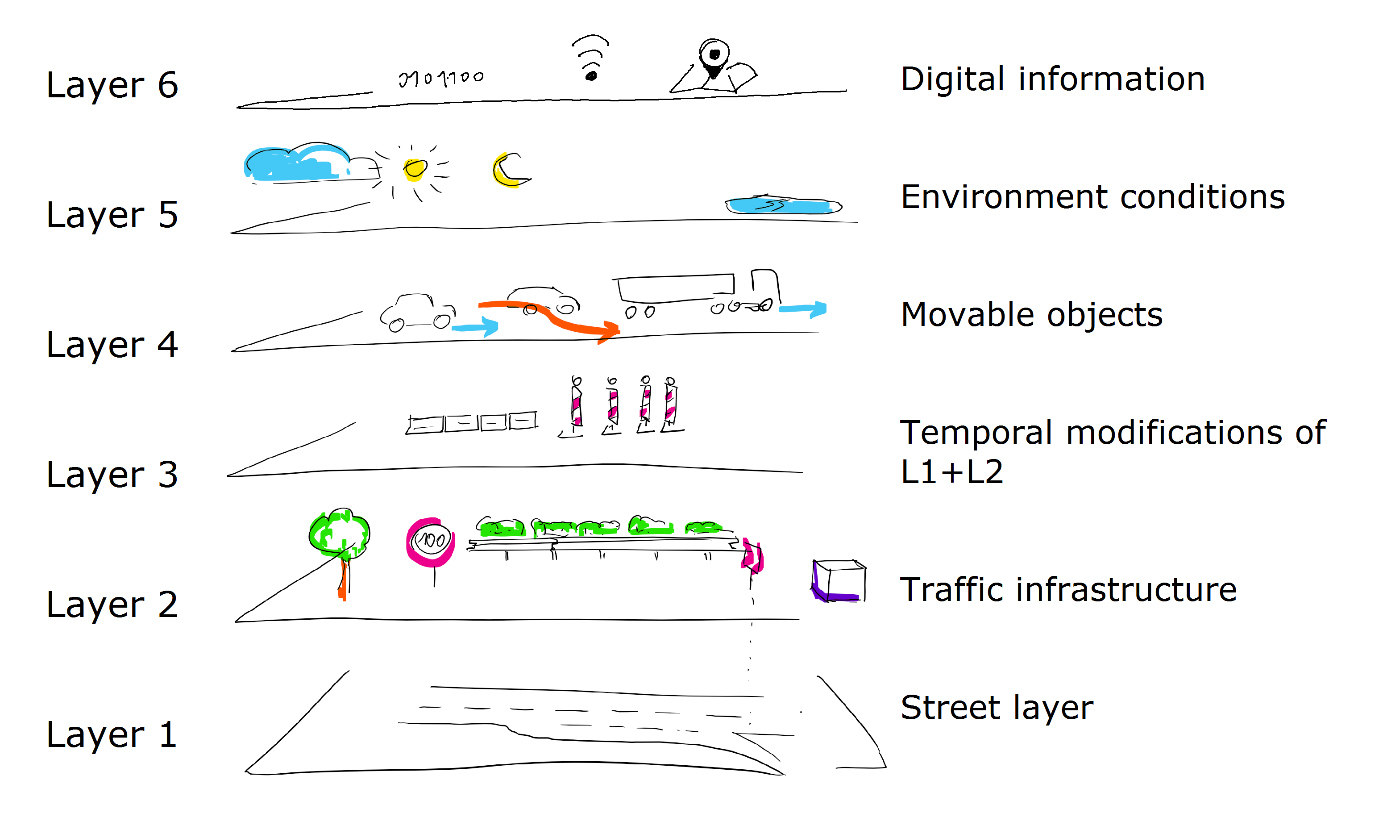
\includegraphics[width=0.95\textwidth]{fig/fig1.png}
	\caption{Test \cite{Donges.1982,Werling.2017}}
	\label{abb1}
\end{figure}

Im Allegemeinen gibt es zwei relevante Koordinatensysteme für Strecken. Neben dem globalen x-y Koordinatensystem existiert das der Referenzlinie mitbewegte s-t Koordinatensystem, wie auch Abbildung \ref{abb2} verdeutlicht. Jede Straße besitzt eine Referenzlinie, deren Beschreibung analytisch durch das Verbinden von Gerade, Kreisbögen und Spiralsegmenten möglich ist. Diese im Straßenbau standardisierte Methode ermöglicht eine kontinuierliche Beschreibung ohne Krümmungssprung, ebenfalls in Abbildung \ref{abb2} zu entnehmen. Eine Gerade mit Krümmung Null und ein Kreisbogen mit konstanter Krümmung können durch ein Sprialsegment mit linearem Krümmungsanstieg verbunden werden.

\begin{figure}[h]
	\flushleft
	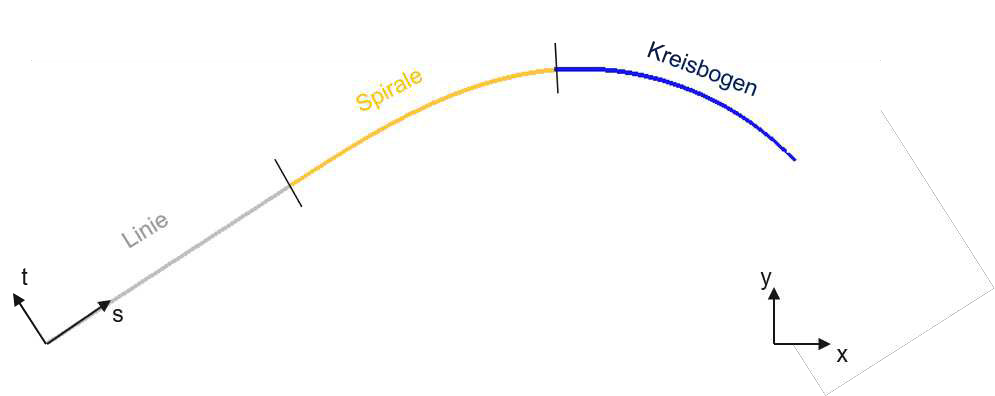
\includegraphics[width=0.95\textwidth]{fig/fig2.png}
	\caption{Test \cite{Donges.1982,Werling.2017}}
	\label{abb2}
\end{figure}

An die definierte Referenzlinie können im Anschluss dann Fahrbahnen hinzugefügt werden, für welche individuelle Breiten oder Markierungen festgelegt werden können. So wird eine eindeutige Streckenbeschreibung möglich und gewährleistet.

% --- OPEN DRIVE STANDARD ------------------------------------------------------
\chapter{OpenDrive Standard}
%\thispagestyle{ika}

OpenDrive ist ein 2006 entwickeltes Format zur Darstellung von logischen Straßennetzwerken und mittlerweile ein Standard für Strecken für Fahrzeugsimulationen. Das Format enthält nicht nur Straßen und Fahrbahninformationen sondern ermöglicht auch die Definition komplexerer Beschilderungen, Fahrbahnmarkierungen oder Ampelsignale. Definiert wird die openDrive Datenstruktur im XML-Format in welcher grundsätzlich zwischen Straßen (\texttt{roads}) und Kreuzungen (\texttt{junctions}) unterschieden wird. Eine vereinfachte Übersicht der openDrive Struktur lässt sich in Abbildung\ref{abb3} finden. Die Refenzlinie wird wie erläutert mit Segmenten analytisch beschrieben, wobei zusätzlich die laterale Position und Ausrichtung sowie das Höhenprofil der Straße definiert werden können. Hinzugefügt werden dann einzelne Fahrbahnen (\texttt{lanes}). An Kreuzungen werden die Fahrbahnverbindungen zwischen unterschiedlichen Straßen als eigene Straßen definiert. Diese können dann im openDrive Format über \texttt{junctions} miteinander verbunden werden. Zudem lassen sich unbegrenzt Objekte definieren. Dies sichert eine eindeutige und korrekte Beschreibung der gewünschten Strecke, macht das XML-Format allerdings auch sehr komplex und für einen Nutzer von Hand kaum generierbar.

\begin{figure}[h]
	\flushleft
	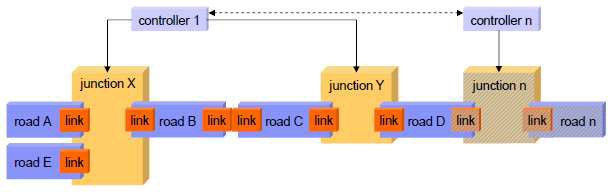
\includegraphics[width=0.95\textwidth]{fig/fig3.png}
	\caption{Test \cite{Donges.1982,Werling.2017}}
	\label{abb3}
\end{figure}

Deshalb existieren Tools mit denen ermöglicht wird eine Strecke über eine grafische Benutzeroberfläche im openDrive Format zu erzeugen. Zur Abbildung der Realtität kann dies herangezogen werden, allerdings ist die generische Varierbarkeit von Strecken ein grosser Vorteil bei der Simulation von Fahrmanövern die zur Absicherung durchgeführt werden.

% --- ANNAHMEN UND VEREINFACHUNGEN IM IKA KONZEPT ------------------------------
\chapter{Annahmen und Vereinfachungen im ika Konzept}
%\thispagestyle{ika}

Um eine logisch varierbare Straße im openDrive Format zu erzeugen, bedarf es ein Tool dass anhand eines vereinfachten, benutzerfreundlichem Eingabeformat das komplexe, detailreiche openDrive Format generiert. Das Konzept dieses Eingabeformats und die dazugehörigen Vereinfachungen werden in diesem Abschnitt erläutert.

Anders als im openDrive Format werden Kreuzungen vom Nutzer nur über die Ausgangsstraßen und einem gemeinsamen Kreuzungspunkt definiert, die definition der Verbindungsstraßen im Kreuzungsbereich sind nicht notwendig. Der Nutzer spezifiziert lediglich Parameter wie die miteinander zu verbindenen Fahrbahnen oder die Größe des Kreuzungsbereichs. Auch werden Spuraufweitungen für Linksabbiegerspuren auf Hauptstraßen angenommen oder Fahrbahnmarkierungen innerhalb des Kreuzungsbereich automatisiert bestimmt. Die Vielfalt bei der Generierung von Kreuzungen ist dadurch zwar eingeschränkter, jedoch für die Simulationen von Fahrmanövern ausreichend. So können durch wenige Paramteränderungen wie beispielsweise dem Schnittwinkel der zwei Straßen einer X-Kreuzung schnell beliebig viele, unterschiedliche und valide Kreuzungen generiert werden. 

Zudem muss der Benutzer keine expliziten Koordinaten der Straßen angeben, da die Annahme getroffen wird, dass der Kreuzungsmittelpunkt im x-y Ursprung liegt. Darüber hinaus gibt es die Möglichkeit verschiedene Kreuzungssegmente über zwei klar definierte Straßenpunkte miteinander zu verbinden. Über die x-y Koordinaten und den Winkel der Straße ist die Lage der beiden Segmente eindeutig spzifiziert. Das Verbinden von mehreren Elementen ermöglicht so ein vorheriges unabhängiges definieren. 

Um ein Straßennetzwerk schliessen zu können bedarf es einer sehr genauen Konstuktion des letzten Segmentes, welches sich in einem überbestimmten Problem wiederspiegelt. Deshalb wird zum Schliessen eines Netzwerks eine separate Funktion entwickelt, die zwei Punkte unter entsprechendem Winkel miteinander verbindet. Dabei wird angenommen, dass die genaue Geometrie eines letzen Segments nicht von grosser Bedeutung ist.

Für den Nutzer sind also nur vereinfachte Angaben wie der Krezungstyp, die Straßengeometrie, der Kreuzungsschnittwinkel oder die Fahrbahnanzahl gefragt. Die Aufgabe des Tools ist nun die Übersetzung in ein detaillreiches Straßennetzwerk im gängigen openDrive-Format.

% --- UMSETZUNG UND IMPLEMENTIERUNG DES TOOLS ----------------------------------
\chapter{Umsetzung und Implementierung des Tools}
%\thispagestyle{ika}

\section{Ein - und Ausgabeformat}
Die Definition im vereinfachten Eingabeformat geschieht ebenfalls wie die Darstellung des openDrive Formats in einer XML-Struktur. Dies erlaubt eine übersichtliche Defintion der Datenstruktur mit Hilfe von Attributen und Elementen. Das Tool zur Generierung des openDrive-Formats wird in c++ geschrieben, sodass eine kompatible Bibliothek zum einlesen und schreiben der XML-Dateien verwendet wird. Die Bibliothek \texttt{pugi\_xml} ermöglicht das Einlesen der Eingabedatei und speichert die XML Struktur ähnlich einer Baumstruktur zur Laufzeit, was entsprechend eine effiziente und übersichtliche Verwendung der Eingaben innerhalb des Tools ermöglicht. Ebenso wird eine solche XML-Stuktur zur Laufzeit des Tools erzeugt, die dann mit den generierten openDrive Obejekten gefüllt werden kann. 

Ein weiterer Vorteil bei der Benutzung von XML Datenstrukturen ist die Möglichkeit von XML Schemata (XSD). Eine \texttt{.xsd} Datei beschreibt die Struktur eines XML Dokumentes, sodass das Vorkommen von Attributen und Elementen eingeschränkt werden kann. So besteht beispielsweise die Möglichkeit die Anzahl von Elementen einzuschränken, die Anordnung von Elementen innerhalb des XML Dokuments vorzuschreiben oder Attribute nur optional vorzuschreiben. So wurde im Rahmen der Seminararbeit ein XML-Schema Dokument zur Absicherung von falschen Benutzereingaben erstellt. Das openDrive Format besitzt ebenfalls eine solche Schemadatei, sodass sowohl Eingabe als auch Ausgabedokument des Streckengenerators mit Hilfe eines XML/XSD Validierungstools abgesichtert werden können.
 
\section{Implementierung}
Die Implementierung des in \texttt{C++} entwickelten Tools gliedert sich ebenfalls in die drei schamtisch beschriebenen Entwicklungsschritte. Im ersten Schritt werden die Segmente (Kreuzungen, Kreisverkehre oder Verbindungsstraßen) miteinander verbunden. Im Anschluss werden diese Segmente dann wie von Benutzer definiert miteinader verbunden bevor im letzten Schritt Straßen zum schliessen des Streckennetzwerkes generiert werden.

\subsection{Generierung der Segmente}
Die Eingabedaten werden zur Laufzeit eingelesen und sind so global als Baumstruktur verfügbar. Im folgenden wird der Entwicklungsprozess einer X-Kreuzung genauer beschrieben. 

Für eine X-Kreuzungen existieren drei verschiedene Fälle wie in Abbildung \ref{abb4} dargestellt, welche sich in Anzahl und Anordnung der definierten Eingangsstraßen unterscheiden.

\begin{figure}[h]
	\flushleft
	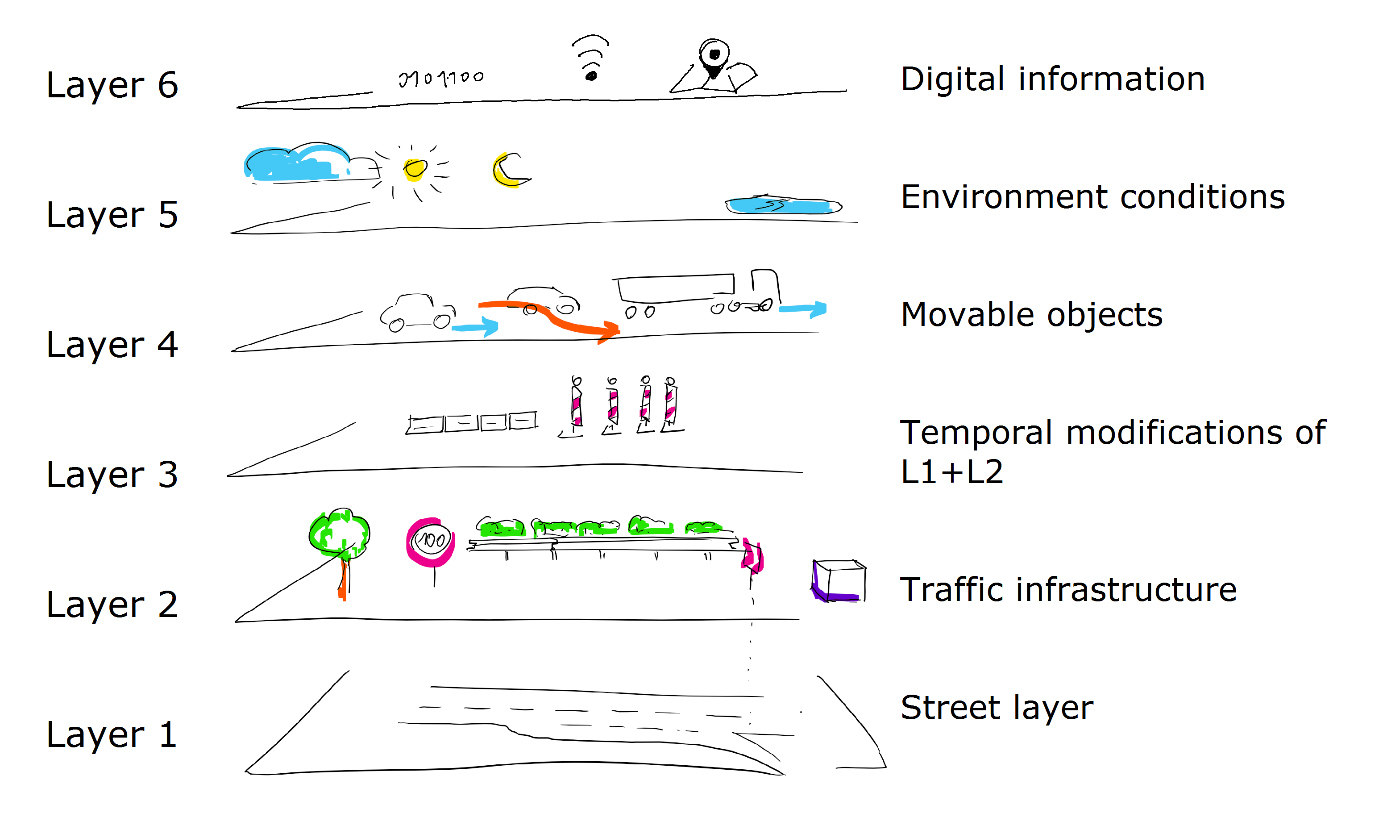
\includegraphics[width=0.95\textwidth]{fig/fig1.png}
	\caption{Test \cite{Donges.1982,Werling.2017}}
	\label{abb4}
\end{figure}

Abhängig vom definierten Kreuzungstyp werden die entsprechend relevanten Strassen und die zugehörigen Informationen wie beispielsweise die Kreuzungsbereichgröße aus dem XML Dokument eingelesen. Im nächsten Schritt werden vier Ausgangsstrassen der X-Kreuzung basierend auf den Eingangsstraßen generiert, welche sich entsprechend dem definierten Winkel schneiden. Die generische Funktion \texttt{generateRoad} erstellt dabei eine Straße ausgehend vom bestimmtem Hauptpunkt im Kreuzungsbereich. Die positive s Koordinatenrichtung zeigt dabei immer weg vom Kreuzungsmittelpunkt. 

Nach erfolgreicher Erstellung der vier Ausgangsstrassen werden die Strassen im Kreuzungsbereich erstellt. Der Benutzer hat die Möglichkeit alle Fahrbahnen automatisch und logisch miteinander zu verbinden oder selbst Verbindungsstraßen zu spezifizieren. Beim definieren einer Fahrbahn ist darauf zu achten, dass sich mögliche Unterschiede im T-Offset oder der Spurbreite kontinuierlich ausgleichen. Die Funktion \texttt{createRoadConnection} verbindet diese Funktionen miteinander und generiert eine Verbindungsstrasse mit vorgegebener Fahrbahnmarkierung. 

Im Kreuzungsbereich besitzt jede angelegte Strasse als Vor und Nachfolger eine \texttt{connection}, welche ebenfalls innnerhalb der Funktionen festgelegt und definiert werden. Die zugrundeliegende Struktur lässt sich nochmals in Abbildung \ref{abb3} erkennen.

Analog werden auch die weiteren Segmente wie beispielsweise eine T-Kreuzung, ein Kreisverkehr oder auch eine einfache Verbindungsstrasse generiert und abgespeichert.

\subsection{Anordnung der Segmente}

Durch den Benutzer wird in der Eingabedatei das Referenzsegment mit Position festgelegt. Alle Geometrien diese Segements werden also innerhalb des Tools um den definierten Winkel gedreht und um x-y Achse verschoben, sodass sich der Urspung des Segments (Kreuzungsmittelpunkt) an definierter Position befindet.

Weiterhin gibt der Nutzer Strassenpunkte zweier unterschiedlicher Segmente an, die miteinader verbunden werden sollen. Innerhalb der Funktion \texttt{linkSegments} wird dann der Winkel um den gedreht werden muss und die x-y Werte der Verschiebung bestimmt, sodass nach Transformation der Geometrien des neuen Segments die Punkte der zwei Strassen ohne Winkelsprung aufeinander liegen. 

\subsection{Verbinden der Segmente}

Im letzten Schritt werden automatisch Straßen generiert, die zwei beliebige Punkte miteinader verbinden, was im Entwicklungsprozess zum Schließen eines Streckennetzwerkes erforderlich ist. Die verantwortliche Funktion \texttt{closeRoadConnection} berechnet hierbei aus den Koordinaten und Richtungen der Punkte die Verbindungsstrecke. Dazu wird der Schnittpunkt der beiden Richtungsvektoren gebildet und unterschieden, ob der Schnittpunkt auf positiver oder negativer Seite des Punktes liegt. Dies führt letztendlich zu neun verschiedenen Fällen, je nach Ausrichtung der beiden zu verbindenen Punkte. Falls eine direkte Verbindung mit Hilfe einer Gerade und einer Verbundkurve nicht möglich ist wird ein Hilfspunkt eingefügt, die Strecke bis dahin mit Gerade oder Kreisbogen erweitert und entsprechend mit den neuen Punkten die Funktion \texttt{closeRoadConnection} rekursiv aufgerufen. Der Fall, dass die Punkte direkt miteinander verbunden werden können lässt sich in zwei Fälle teilen.

Zum einen ist dies möglich falls beide Vektoren in die gleiche Richtung und der Startvektor auf den Endvektor zeigt. Für diesen trivialen Fall lässt sich das Stück mit einer einfachen Geraden verbinden. 

Für den Fall, dass der Schnittpunkt in positiver Richtung des Startvektors und in negativer Richtung des Endvektors liegt lässt sich die Strecke ebenfalls verbinden. Dazu wird das der Abstand von Start und Endpunkt zum Schnittpunkt verglichen und das längere Stück soweit mit einer Geraden verlängert, bis Start und Endpunkt gleichweit entfernt liegen. Nun lässt sich das fehlende Stück mit Hilfe eines Kreisbogens schliessen. Für kleine Geschwindigkeiten wird hierbei der Krümmungssprung zwischen Gerade und Kreisbogen toleriert. Die Berechnung des Kreisbogens erfolgt mit Konstruktion eines Gleichschenkligem Dreieck wie in Abbildung \ref{abb5} dargstellt. 

\begin{figure}[h]
	\flushleft
	\includegraphics[width=0.95\textwidth]{example-image}
	\caption{Test \cite{Donges.1982,Werling.2017}}
	\label{abb5}
\end{figure}

Daraus lässt sich über die Beziehung 

\begin{align}
    \begin{equation}
        sin(\frac{\alpha}{2) = \frac{\frac{d}{2}}{R}
    \end{equation}
\end{align}

der Kreisradius und mit dem Winkel \(\alpha\) ebenfalls die Länge des Kreissegments berechnen. Somit ist der Kreis, welcher die fehlende Lücke schliesst klar definiert und das Strassensegment geschlossen.

Für den Fall, dass die Strasse an Start oder Endpunkt eine Krümmung besitzt wird automatisch ein Sprialsegment eingefügt, welches den Krümmungssprung überbrückt. Ähnliches gilt, falls die Anzahl der Spuren oder die Breite von Start und Endpunkt variert.

Das vorgehen gewährleistet einen kontinuierlichen Übergang vom Starpunkt in den Endpunkt und somit ein korrektes Schliessen des Strassennetzwerkes. Zusammen mit den anderen gezeigeten Funktionen bildet das Tool also eine Möglichkeit beliebige Strassennetze zu konstruieren und im openDrive Format abzuspeichern. Diese sind dann nutzbar für weitere Simulationen.

% --- BEISPIELE UND TESTS ------------------------------------------------------
\chapter{Beispiele und Tests}
%\thispagestyle{ika}

Im folgenden Abschnitt finden sich einige beispielhafte generierte Kreuzungen. Zudem wurden im letzten Schritt einige zuvor generierte Strassen zusammengefügt und durch Verbindungsstrassen mit Hilfe der Funktion \texttt{closeRoadConnection} geschlossen. 

\section{X-Kreuzung}
Wie schon erläutert gibt es für Kreuzungen verschiedene Typen. Der hier beispielhaft gezeigte Typ besteht aus einer durchgehenden Hauptstrasse und zwei aneinandergrenzenden Nebenstrassen. Verbunden werden sollen alle Fahrstreifen im Kreuzungsbereich und die Kreuzungsbereichgröße wird auf 15m in alle Richtungen gesetzt. Per Definition befindet sich der Kreizungsmittelpunkt im Ursprung des xy Koordinatensystems. Eine Darstellung der beispielhaften Krezung befindet sich in Abbildung \ref{abb6}.

\begin{figure}[h]
	\flushleft
	\includegraphics[width=0.95\textwidth]{example-image}
	\caption{Test \cite{Donges.1982,Werling.2017}}
	\label{abb6}
\end{figure}

Annahme innerhab des Tools ist, dass Hauptstrassen eine zusätzliche Linksabbiegerspur besitzen welche in der Abbildung sichtbar wird. Durch einen hier im Beispiel sehr grossen Kreuzungsbereich werden die einzelnen Spuren auch ohne Fahrbahnmarkierung gut sichtbar. Automatisiert werden alle relevanten Spuren miteinander verbunden. Das Beispiel zeigt also eine valide Kreuzung generiert aus einfachen Eingabedaten.

\section{Kreisverkehr}
Analog zur X-Kreuzung kann ein Kreisverkehrsegment erstellt werden. Ausgangspunkt ist die Definition des Kreises, der angrenzenden Strassen und jweils die Position und der Winkel des Schnittpunkts. Daraus generiert das Tool alle Kreuzungsbereiche des Kreisverkehrs eigenständig, schneidet die das Kreissegment an den entsorechenden Stellen und erstellt die Verbindungsstraßen der einzelnen Kreuzungen. Eine Visualisierung der Straßen lässt sich in Abbuldung \ref{abb7} finden.

\begin{figure}[h]
	\flushleft
	\includegraphics[width=0.95\textwidth]{example-image}
	\caption{Test \cite{Donges.1982,Werling.2017}}
	\label{abb6}
\end{figure}

Angrenzend an eine ringförmige Straße treten vier Nebenstraßen auf, die zsammen  mit Verbindungsstrassen in einem geschlossenen, in sich validem Kreisverkehr resultieren.   

\section{Komplexes Straßennetzwerk}

Diese und weitere parametrisierte Segmente lassen sich mitHilfe des erstellen Tools generieren. Das zugrundeliegende Beispiel zeigt nun, dass die Segmente aneinander gefügt werden können und ferner zwei Straßenenden mit einer neu generierten Straße automatisiert miteinander Verbunden werden können. Zwar ist die erstellte Verbindungsstrasse nicht immer die kürzeste Möglichkeit zur Verbindung der Strassen, jedoch wird der genaue Verlauf der Verbindungsstraße hierbei auch vernachlässigt.

\begin{figure}[h]
	\flushleft
	\includegraphics[width=0.95\textwidth]{example-image}
	\caption{Test \cite{Donges.1982,Werling.2017}}
	\label{abb7}
\end{figure}

Zudem zeigt das Beispiel, welches in Abbildung  \ref{abb7} zu finden ist weitere Funktionen des Tools, wie beispielsweise Spuraufweitungen oder einen Ausgleich von unterschiedlichen Spurbreiten.

Insgesamt zeigen die dargstellten Beispiele, dass das Tool die vereinfachten Eingaben des Nutzers, zusammen mit Annahmen in ein valides und generisches Straßennetz im openDrive Standard erstellt.

% --- AUSBLICK -----------------------------------------------------------------
\chapter{Ausblick}
%\thispagestyle{ika}

Das in dieser Seminararbeit entwickelte Tool ermöglicht es mit Hilfte einer vereinfachten Streckenbeschreibung ein vollständiges Streckennetz im standardisierten openDrive Format zu generieren. Dies erlaubt Benutzern durch einfache Paramteränderungen komplett unterschiedliche, aber valide Strecken zu erhalten. So ist es möglich grosse Strecken mit wenigen Eingaben zu generireren und für eine anschliessende Simulation zu benutzen.

Im Rahmen der Arbeit wurde der Streckengenerator in \texttt{C++} entwickelt und die Grundfunktionen implementiert. Selbstverständlich können aber weitere Annahmen getroffen werden und so eine noch intuitivere und einfachere Eingabe des Benutzers sicher gestellt werden. Zudem können weitere Funktionen eingebaut werden, die dann weitere Szenarien abdecken. Beispiele hierfür sind Verkehrsinseln, Fußgängerüberwege, Parklücken oder Bushaltestellen. Letzendlich ist durch das offen gehaltene openDrive Format jedes mögliche Szenario auch mit Hilfe des Generators in openDrive umsetzbar.

